\documentclass{article}
\renewcommand\refname{Referencias}
\renewcommand\contentsname{\'Indice de Conten\'ido}
\usepackage{graphicx}
\graphicspath{{IMG/}}
\usepackage{caption}
\usepackage{subcaption}
\usepackage{float}
\usepackage{listings}
\lstset{
	morekeywords={MPI\_Init, MPI\_Finalize, MPI\_Send, MPI\_Recv,
MPI\_Comm\_size, MPI\_Comm\_rank},
	language=[11]C++,
	basicstyle=\footnotesize\bfseries\ttfamily,
 	showstringspaces=false,
 	tabsize=2,
 	frame=single,
 	numbers=left
}
\renewcommand{\lstlistingname}{C\'odigo}
\renewcommand{\lstlistlistingname}{Lista de ejercicios de codificaci\'on}

\title{\textsc{Paradigmas y Lenguajes de Programación\\Trabajo Práctico Número
3\\-- Práctica --}}
\author{Ulises C. Ramirez [uli.r19@gmail.com]\\H\'ector Chripczuk\\Gonz\'alez
Ver\'onica}
\date{28 de Septiembre, 2018}
\begin{document}
\maketitle
\pagenumbering{gobble}
\newpage
\section*{C\'odigo}
Todo el c\'odigo que est\'e expresado en el documento como respuesta a alg\'un
ejercicio est\'a contenido en la carpeta \texttt{codigo}, junto a el se podr\'a
encontrar la salida del compilador.

\section*{Versionado}
Para el corriente documento se est\'a llevando un versionado a fin de mantener
un respaldo del trabajo y adem\'as proveer a la c\'atedra o a cualquier interesado
la posibilidad de leer el material en la \'ultima versi\'on disponible.\\

\begin{center}
  \textsc{Repositorio}: \textit{https://github.com/ulisescolina/UC-PYLP}
\end{center}

\hfill--\textsc{Ulises}
\tableofcontents
\pagenumbering{gobble}
\newpage

% === Inicio del Cuerpo del Documento === %
\pagenumbering{arabic}
\section{Ejercicio 1}
\label{sec:ej1}
\textsc{Consigna}: \textbf{resolver el ejercicio planteado en la página de la
\cite{unigranada}, Tutorial 01 Hello World.
\begin{itemize}
\item Explique brevemente como funciona el c\'odigo fuente.
\item Describa las instrucciones propias de MPI utilizadas en el ejercicio.
¿Cuáles son los parámetros de entrada y cuáles son los parámetros de salida?
\end{itemize}}

En primera instancia, accedemos a la página brindada por la cátedra, y
obtenemos un archivo base con el cual trabajar.

\lstinputlisting[caption={C\'odigo base para Hello World desde \cite{unigranada}},
label=lst:base]{codigo/punto_1_base.cpp}

De ahora en adelante se eliminan las primeras 10 lineas del código expuesto en
\texttt{C\'odigo \ref{lst:base}}, dado a que simplemente son comentarios, la
razon de que se los haya presentado es porque estos demuestran los datos del creador.

La página tiene desde ya una ayuda que permite conocer que sentencias se
necesitan para la correcta implementacion de lo que solicita el ejercicio. Se
menciona que los necesario para un funcionamiento minimo de \texttt{OpenMPI}
son las siguientes instrucciones, según \cite{pylp32018}:
\begin{itemize}
\item \textbf{MPI\_Init}: este comando inicializa el entorno MPI.
\item \textbf{MPI\_Finalize}: finaliza el entorno de MPI.
\item \textbf{MPI\_Comm\_size}: determina la cantidad de procesos del
comunicador.
\item \textbf{MPI\_comm\_rank}: representa el id de un proceso.
\end{itemize}

La implementación de lo solicitado se puede ver en el \texttt{Código
\ref{lst:mpi1}}, la explicación de cada linea se presenta luego.

\lstinputlisting[language=C++, caption={Soluci\'on ejercicio 1},
label=lst:mpi1]{codigo/punto_1_mpi.cpp}

Para informaci\'on acerca de la compilaci\'on del archivo, junto a una
explicaci\'on relacionada a la \texttt{L\'inea 2} del \texttt{C\'odigo
\ref{lst:mpi1}} puede revisar lo presentado en el \texttt{Anexo \ref{an:compilacion}}

Las diferencias con el \texttt{C\'odigo \ref{lst:base}} inician en la linea
\texttt{10}, aqu\'i definimos variables en las cuales vamos a guradar
informaci\'on acerca de lo que va sucediendo a medida que se ejecuta el
c\'odigo, es importante aclarar que estas variables son globales y estan
disponibles para todas las instancias de los procesos, de esta forma los mismos
pueden comunicarse. En la l\'inea \texttt{11} iniciamos con lo relacionado a MPI, aqu\'i
se inicializa el entorno, mediante \texttt{MPI\_Init}, en la l\'inea \texttt{12}
se establece un tamaño para el \textit{comunicador} (lugar que contiene, por
defecto, todos los procesos), consecuentemente, esto dar\'a la cantidad de
procesos a ser instanciados. en la siguiente l\'inea, lo que se hace es obtener
el \texttt{id} del proceso actual, teniendo esta informaci\'on ya podemos
empezar a imprimir lo que nos solicita el ejercicio, esto se hace en las l\'ineas
\texttt{14} y \texttt{15}, y por \'ultimo se finaliza en la l\'inea \texttt{16}
con el entorno MPI.

\section{Ejercicio 2}
\label{sec:ej2}
\textsc{Consigna}: \textbf{Queremos hacer un programa paralelo que encadene el
envío y recepción de un mensaje, en nuestro caso el mensaje sera el rango
(identificador) del proceso que envía.
Los mensajes se enviarán de forma encadenada, lo que quiere decir que el
primero enviará un mensaje al segundo, el segundo recibirá uno del primero y
enviará uno al tercero, y así sucesivamente para todos los procesos lanzados.
Todo proceso que reciba un mensaje debe imprimirlo de la forma "Soy el proceso
X y he recibido M", siendo X el rango del proceso y M el mensaje recibido.
}\\

Antes de presentar el c\'odigo cabe mencionar que la consigna no se sigue al
pie de la letra, se modifica un poco en cuanto al valor que envia, siendo este
la variable \texttt{mensaje} la cual es un entero que se define a la hora de
mandarla la primera vez. Y luego se reenv\'ia el mismo entero pero se le
adiciona una unidad es decir \texttt{mensaje + 1}.

\lstinputlisting[caption={Soluci\'on ejercicio 2},
label=lst:mpi2]{codigo/punto_2_mpi.cpp}

Los conceptos principales dentro del entorno MPI vistos en este ejercicio son
dos, \texttt{MPI\_Send} y \texttt{MPI\_Recv}, estos complementan a los comandos
introductorios vistos en la \texttt{Secci\'on \ref{sec:ej1}}, y la utilidad que
proveen es la de enviar y recibir mensajes respectivamente. La utilizaci\'on
con respecto a la sint\'axis y errores que se pueden esperar arrojen los
comandos en cuesti\'on est\'an explicados en la p\'agina de la \cite{unigranada} en
el apartado correspondiente para MPI\_Send y MPI\_Recv, y \cite{pylp32018}. Para
no ser redundante, ac\'a solo se va a explicar que est\'a haciendo cada uno de
ellos en el \'ambito que propone el ejercicio.

\begin{lstlisting}[caption={ Fragmento de \texttt{C\'odigo \ref{lst:mpi2}}},
label=lst:snp:1, firstnumber=18]
	if (id == 0)
\end{lstlisting}

Lo expuesto anteriormente en el \texttt{C\'odigo \ref{lst:snp:1}} es una
enseñanza tomada de c\'atedras como Sistemas Operativos, en la cual tratabamos
con procesos y era de vital importancia conocer su \texttt{id}, aqui es igual
de importante, comenzando por lo solicitado en el ejercicio se sabe que no se
desea tener un \texttt{anillo} de procesos, m\'as bien se prefiere una simple
\texttt{cola} de ellos como se representa en \texttt{Figura \ref{fig:conej2}}.

\begin{figure}[H]
  \centering
  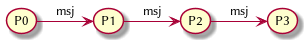
\includegraphics[width=.4\linewidth]{EJ2}
  \caption{Concepto de lo requerido en el Ejercicio 2}
  \label{fig:conej2}
\end{figure}

Entonces, es vital que conozcamos cual es el proceso \texttt{P0} en este caso,
dado a que este no debera recibir nada, unicamente enviar\'a un mensaje al
siguiente proceso y eso concluir\'a con su tarea, que es exactamente lo que
est\'a pasando en el \texttt{C\'odigo \ref{lst:snp:2}}

\begin{lstlisting}[caption={MPI\_Send para P0 - Fragmento de \texttt{C\'odigo \ref{lst:mpi2}}},
label=lst:snp:2, firstnumber=19]
		mensaje = 1000;
		MPI_Send(&mensaje, /* Mensaje a enviar */
			1, /*Cantidad de elementos*/
			MPI_INT, /* Tipo de dato del mensaje*/
			id+1, /*Proceso receptor del mensaje*/
			0, /* Etiqueta del mensaje */
			MPI_COMM_WORLD /* Comunicador */);
\end{lstlisting}

All\'i evidenciamos lo que realiza el proceso \texttt{P0} (conceptualizaci\'on
presentada en la \texttt{Figura \ref{fig:conej2_1}}), inicializamos una
variable \texttt{mensaje=1000} que ser\'a lo que enviaremos, al siguiente
proceso que sera el proceso \texttt{P1} ya que est\'a representado por
\texttt{id+1} en el proceso con id=0, luego este proceso concluir\'a
diciendonos que envi\'o dicho valor que declaramos, junto a su id, el de su destinatario, y que no
debe realizar ninguna acci\'on m\'as.

\begin{figure}[H]
  \centering
  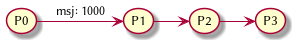
\includegraphics[width=.4\linewidth]{EJ2_001}
  \caption{Conceptualizaci\'on de \texttt{C\'odigo \ref{lst:snp:2}}}
  \label{fig:conej2_1}
\end{figure}

Siguiendo por el \texttt{else} del \texttt{if} presentado en el
\texttt{C\'odigo \ref{lst:snp:1}} tendremos el  siguiente c\'odigo que lo vamos
a presentar en 2 partes, en la primera vamos a ver otro de los conceptos que nos
ocupan en la secci\'on y en la segunda vamos a tratar con lo mismo que tratamos
cuando hablamos del proceso \texttt{P0}.

\begin{lstlisting}[caption={ 1ra parte MPI\_Recv - Fragmento de \texttt{C\'odigo \ref{lst:mpi2}}},
label=lst:snp:3, firstnumber=29]
		MPI_Recv(&buzon, /* Almacenamiento de msj */
			 1, /* Cantidad de elementos
				que se esta recibiendo */
			 MPI_INT, /* Tipo de dato a recibir*/
			 id-1, /* id del proceso origen */
			 0, /* Etiqueta esperada para msj */
			 MPI_COMM_WORLD, /* Comunicador utilizado */
			 &estado /* Info del estado */);
\end{lstlisting}

El \texttt{C\'odigo \ref{lst:snp:3}} presenta la aplicaci\'on de
\texttt{MPI\_Recv}, y lo que se est\'a haciendo es guardando lo que envi\'o
P0 como se demuestra en la \texttt{Figura \ref{fig:conej2_1}}, y lo est\'a
almacenando en una variable que se denomi\'o \texttt{buzon}, se representa el
curso de  acci\'on en la \texttt{Figura \ref{fig:conej2_2}}.

\begin{figure}[H]
  \centering
  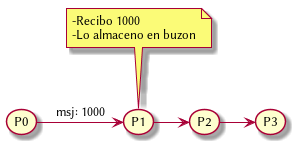
\includegraphics[width=.4\linewidth]{EJ2_002}
  \caption{Conceptualizaci\'on de \texttt{C\'odigo \ref{lst:snp:3}}}
  \label{fig:conej2_2}
\end{figure}

Ahora se prosigue con la segunda parte de la explicaci\'on e iniciamos
pregunt\'andonos que significa la condici\'on en el \texttt{C\'odigo \ref{lst:snp:4}}

\begin{lstlisting}[caption={Condici\'on para detectar \'ultimo proceso},
label=lst:snp:4, firstnumber=37]
	if (id != tamanio-1)
\end{lstlisting}

Recordando la \texttt{Figura \ref{fig:conej2}}, y el hecho de que no se
necesita un anillo para el ejercicio, es necesario saber cual es el \'ultimo
nodo, adem\'as de conocer el primero, esto se logra mediante el \texttt{C\'odigo \ref{lst:snp:4}}
en este caso, y a diferencia del primero, el \'ultimo nodo recibe un mesaje del
nodo predecesor, pero no comunica ninguno.
Esta acci\'on se codific\'o de la siguiente manera

\begin{lstlisting}[caption={ 2da parte MPI\_Recv - Fragmento de \texttt{C\'odigo \ref{lst:mpi2}}},
label=lst:snp:5, firstnumber=38]
			mensaje = buzon+1;
			MPI_Send(&mensaje, /* Mando mensaje que recibo */
				1, /*Cantidad de elementos*/
				MPI_INT, /* Tipo de dato del mensaje*/
				id+1, /*Proceso receptor del mensaje*/
				0, /* Etiqueta del mensaje */
				MPI_COMM_WORLD /* Comunicador */);
			realiza_envio = true;
\end{lstlisting}

Conceptualizando el \texttt{C\'odigo \ref{lst:snp:5}}, se concluye con un
escenario como lo presentado en la \texttt{Figura \ref{fig:conej2_3}}.

\begin{figure}[H]
  \centering
  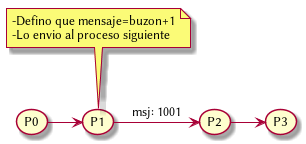
\includegraphics[width=.4\linewidth]{EJ2_003}
  \caption{Conceptualizaci\'on de \texttt{C\'odigo \ref{lst:snp:5}}}
  \label{fig:conej2_3}
\end{figure}

\texttt{realiza\_envio} es una variable booleana que permite tener idea de si,
el proceso que se est\'a ejecutando envi\'o algo o solo recibi\'o algo, de esta
manera se puede mostrar un mensaje mas personalizado a la hora de la
ejecuci\'on del c\'odigo.

Para finalizar se muestra una captura con el c\'odigo ejecutado en 4 procesos.

\begin{figure}[H]
  \centering
  \includegraphics[width=.95\linewidth]{EJ2_Captura}
  \caption{Captura de pantalla de la ejecuci\'on del \texttt{C\'odigo \ref{lst:mpi2}}}
  \label{fig:ej2_captura}
\end{figure}

\section{Ejercicio 3}
\label{sec:ej3}
\textsc{Consigna}: \textbf{adapte el ejercicio 2, al siguiente planteamiento,
el proceso 0, env\'ia dos mensajes un mensaje \texttt{11111} al proceso 1 y un
mensaje \texttt{22222} al proceso 2, luego el mensaje \texttt{11111} debe ir
pasando por los procesos impares y el mensaje \texttt{22222} debe ir pasando
por los procesos pares.}

\lstinputlisting[caption={Soluci\'on al \texttt{Ejercicio
\ref{sec:ej3}}},label=lst:mpi3]{codigo/punto_3_mpi.cpp}

A continuacion se presenta una captura de pantalla para la ejecucion del
\texttt{C\'odigo \ref{lst:mpi3}}.

\begin{figure}[H]
  \centering
  \includegraphics[width=.95\linewidth]{EJ3_Captura}
  \caption{Captura de pantalla de la ejecuci\'on del \texttt{C\'odigo
\ref{lst:mpi3}}}
  \label{fig:ej3_captura}
\end{figure}



% === Inicio de anexo === %
\newpage
\section{Anexo}
\subsection{Acerca de la compilaci\'on}
\label{an:compilacion}
para la compilación de todo código relacionado con OpenMPI/OpenMP se utilizó el
siguiente script:

\begin{lstlisting}[language=bash, caption={Script de compilaci\'on}]
#!/bin/sh

#Variables globales
# @param $1 archivo con el codigo fuente
# @param $2 nombre base del archivo, sin la extension
archivo=$1
base=$2

# Compila codigo OpenMPI en C++ y lo ejecuta con la cantidad
# de recursos que se le soliciten
compi() {\
 txtcpp=$(sed 10q "$archivo")
 if [[ $txtcpp =~ (NUM_PROC=)([0-9]) ]];
 then
    nproc=${BASH_REMATCH[2]};
 else
    nproc=1;
 fi
 echo && echo
 echo "Compilando el archivo hacia: $base"
 mpicxx "$archivo" -o "$base"
 echo "Corriendo $base con $nproc proceso(s)"
 echo "============ Inicio Ejecucion ================="
 mpirun --oversubscribe -np "$nproc" "$base"
 echo "============== Fin Ejecucion==================="
}

# Compila codigo OpenMP utilizando el compilador para C++,
# luego lo ejecuta
comp(){
 g++ -fopenmp "$archivo" -o "$base" && "$base"
}
\end{lstlisting}

Se aprecian dos funciones una \texttt{copmi()} espec\'ifica para la compilaci\'on
de c\'odigo que necesite los wrappers para OpenMPI, y una segunda denominada
\texttt{comp()} que realiza algo similar, pero para OpenMP.

Una peculiaridad a tener en cuenta, es la forma en la que \texttt{compi()}
trata al archivo, este busca en las primeras 10 lineas una cadena que contenga
lo siguiente: ``NUM\_PROC=\textit{numero\_de\_procesos}'' y lo recuerda. Luego de
ralizar la compilaci\'on del c\'odigo, ejecuta al archivo resultante de
la compilaci\'on mediante \texttt{mpirun -np \textit{«numero\_de\_procesos»
«nombre\_archivo»}} (de no encontrar una expresi\'on con esas caracter\'isticas,
procede a ejecutar el archivo compilado con un solo proceso), lo cual hace que compilaci\'on y
ejecuci\'on se realicen en un solo paso para el usuario.


 % === Bilbiografia === %
\newpage
\begin{thebibliography}{99}
	% Item 1
	\bibitem[Universidad de Granada]{unigranada} \textsc{Universidad de
Granada}. https://lsi.ugr.es/.
	% Item 2
	\bibitem[Clase 3 PyLP - OpenMPI, 2018]{pylp32018}\textsc{Paradigmas y
Lenguajes de Programaci\'on}. \textit{Presentacionde de la Clase 3: OpenMPI}.
\end{thebibliography}
\end{document}
